\documentclass[tikz]{standalone}
\usepackage{bm}
\begin{document}
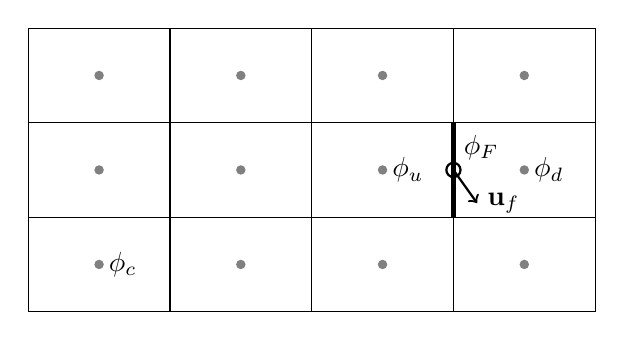
\begin{tikzpicture}[
  scale=0.6,
  cpnt/.style={fill=gray},
]

\draw (0,0) rectangle (12,6);
\draw (0,2) -- (12,2);
\draw (0,4) -- (12,4);
\draw (0,0) -- (0,6);
\draw (3,0) -- (3,6);
\draw (6,0) -- (6,6);
\draw (9,0) -- (9,6);

\draw [ultra thick] (9,2) -- (9,4);
\draw [thick] (9,3) circle [radius=0.15] node [anchor=south west] {$\phi_F$};
\draw [thick, ->] (9,3) -- (9.5,2.3) node [anchor=west] {$\mathbf{u}_f$};

\path [cpnt] (1.5,1) circle [radius=0.1] node [right] {$\phi_c$};
\path [cpnt] (1.5,3) circle [radius=0.1];
\path [cpnt] (1.5,5) circle [radius=0.1];

\path [cpnt] (4.5,1) circle [radius=0.1];
\path [cpnt] (4.5,3) circle [radius=0.1];
\path [cpnt] (4.5,5) circle [radius=0.1];

\path [cpnt] (7.5,1) circle [radius=0.1];
\path [cpnt] (7.5,3) circle [radius=0.1] node [right] {$\phi_u$};
\path [cpnt] (7.5,5) circle [radius=0.1];

\path [cpnt] (10.5,1) circle [radius=0.1];
\path [cpnt] (10.5,3) circle [radius=0.1] node [right] {$\phi_d$};
\path [cpnt] (10.5,5) circle [radius=0.1];

\end{tikzpicture}
\end{document}
